\chapter{Design and Implementation}\label{C:workdone}

\section{Overview}

\todo{REDO ONCE FINISHED SECTION}

\section{Framework}
\label{S:framework}

The spectrum of every test has to be compared to that of every other test in order to identify redundant test cases. The metrics identified become computationally heavy with thousands of test cases containing a spectrum consisting of tens of thousands of methods calls. To perform an analysis on that scale would take several days. A pipeline combined with time reduction strategies was determined to be the best solution.
\paragraph{}
A pipeline approach is shown in Figure \ref{fig:pipeline}. The analysing stages can be set by the user within a properties file, where they can select the spectra type, analysis metric to use and level of redundancy for each. This allows execution of reduction strategies before executing more computationally heavy analysis.

\begin{figure}[h]
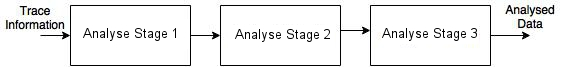
\includegraphics[width=\textwidth]{Pipeline.jpg}
\caption{Trace information goes in at the start of the pipeline. After each stage there will be a reduction of comparisons that the next stage has to complete. The last stages should be the most computationally heavy.}
\label{fig:pipeline}
\end{figure}

There were two approaches that were used to reduce the amount of analysis time. They were - implementing a heuristic and using concurrent execution. 
\paragraph{}
The heuristic looked at the set spectra of method calls, rather than a list. This meant the number of comparisons decreased. Using a 99 percent similarity for the heuristic on the wyc package of Whiley, this decreased the comparisons that the last had to do from 90,902 to 38.

The following illustrates an example of this.

$K,I,T,C,H,E,N \neq K,I,T,E,N,Z $

In this case, the two test cases would not be redundant due to them having a large difference in method calls.

$K,I,T,C,H,E,N \approx K,I,T,C,H,N$

There is a chance that these two may be redundant so it implies more computational heavy analysis should be done, such as analysing the list spectra or calling context. 
\paragraph{}
Concurrent execution was implemented by splitting the test cases up into 8 different parts, each part knew the test cases that it had to compare. A new thread was run to execute the comparisons, making the implementation relatively easy. The concurrent execution lead to a decrease in roughly 2 times the time taken to analyse the spectra's but lead to a trade off in an increased memory usage. This meant concurrent execution was only usable for the smaller bench marks.
Another issue was that for each analysis of a benchmark, the tests had to be rerun, this could take several hours. The solution was to save the spectra data to disk. This ensured that a distributed grid system, explored later, can be used to analyse the data.

\section{Tracing}
\label{S:trace}
David Pearce's language Whiley is written in Java. Therefore it was decided to use Java to trace a tests spectrum. There are two viable options, the Java Debugging Interface (JDI) or AspectJ, as discussed in Section \ref{C:related}. 
\paragraph{}
It was decided to use AspectJ over JDI. AspectJ is easier to choose which methods to record and returns the actual object when retrieving the parameters of the method call allowing for reflection to be used to retrieve the information for every object. JDI was faster to execute, however as there was a very limited amount of document available and the parameters returned were not the actual objects, meaning that standard reflection could not be used to retrieve the values. The decision to use AspectJ was based off this trade off between information and performance. The analysis framework was able to be altered to increase the performance of it, so having the extra information that AspectJ gave was more important than an taking less time to execute. 
\paragraph{}
To get AspectJ to trace the method execution, a point cut was made to record every execution. A simplified version of the aspect is shown in Figure \ref{fig:aspectused}. There are two point cuts within the aspect, the first pointcut is going to be called for every method which has a junit \@Test annotation attached to it. This will then let a static service know that a new test has been started. The second pointcut is used to trace everything but methods attached to \@Test annotation. 
\paragraph{}
The next stage was to weave the point cuts into the benchmark. Using compile time would have meant that each benchmark needed to be recompiled using the aspect compiler. In contrast to load time, which only requires the AspectJ class loader to be passed through a command line argument. The load time was chosen for it's ease of use when working with external benchmarks as it only required AspectJ's class loader to be use.

\subsection{Parameter Values}
The related work in Section \ref{relatedworkRef} explored the statement coverage while ignoring the parameter values that each method was passed. It could be argued that due to knowing the statement path, parameters are irrelevant as you know the path the method will take, and parameters will not add any more information. When using method execution details alone, these become crucial when determining the level of redundancy due to the limited amount of information that the method details alone gives us. 
\paragraph{}
AspectJ gives access directly to the object's that are contained in the parameter values of the method. This allows for reflection to be used to retrieve the objects in a representable state. By using reflection, the fields of the objects can be retrieved and returned in a string. This string is then examined to remove any java object reference location and stored. Initially it was decided to examine primitive types only, this resulted in a very limited number of parameters and did not have the desired effect of decreasing the level of false positives while increasing the time and memory. Changing to reflection allowed for more detailed parameters to be collected. This increases the certainty about the whether two tests are redundant, decreasing the false positives but increasing the time and memory even more than the use of primitives only. 
\paragraph{}
The most common use case would involve the use of parameters therefore it was decided to optimize this through storing the data with parameters. The optimization involved saving the parameters with the trace information. If parameters value is set to false, the parameters have to be split off rather than added on. This means that setting the parameters to false would increase the set up time.

\begin{figure}[h]
\begin{center}
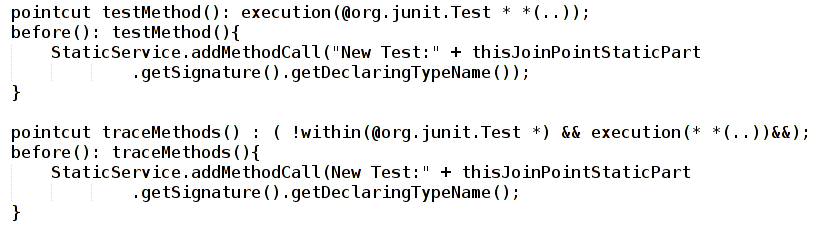
\includegraphics[width = \textwidth]{aspect.png}
\end{center}
\caption{A simplified point cut within AspectJ. The first pointcut is for when a new test is executed and the second when a new method is executed.}
\label{fig:aspectused}
\end{figure}

\section{Test Spectra}
\label{S:spectra}
The idea of a spectrum was previously identified in Chapter \ref{C:intro}. Reexamining the idea, a spectrum is some abstraction of the information that is retrievable during the execution of a test. Our tool is particularly interested in utilising the method execution details. This allows there to be several different types of spectra. The main three spectra examined are \textit{set}, \textit{list} and \textit{calling context}. To explore the different spectra's, an example trace of methods, 'kitten' will be used. Each letter represents a method execution and each letter is executed from the \todo{same parent method}. The different spectra's take up different levels of resources. The resources explored are -- time taken, memory and complexity. 

\subsection{Set}
A set of method executions is where every method execution is only taken into account once. Examining the example trace, the output would be 'kiten', with the difference being the removal of the repeated 't' method. The implication of limiting the method calls to one per method call on the number of comparisons will be dependent the benchmark. Using Whiley Compiler benchmark as an example, there are 494 unique method executions for a single test and 80,000 method calls to these method executions. Utilising the set method, the tool will only examine the 494, rather than the 80,000, a decrease of $\rfrac{6}{1000}$. This leads to a substantial reduction in the time taken and memory used. However, decreasing the amount of data means that there is a decrease in confidence that the tests produced are actual redundant test cases. The motivation behind decreases the resources used and confidence is to use the spectra as a heuristic, as explored in Section \todo{TODO}

\subsection{List}
A list of method executions is where every method execution is taken into account. Examining the example trace, the output would be 'kitten', with there being no difference between the two. Using Whiley Compiler benchmark as an example, a list spectra would examine all 80,000 method calls to calculate the level of redundancy. A list spectra is the same as using a calling context of one, where only the highest method execution is examined. Comparing this to a set spectra, this is expected to lead to an increase in the time taken but increase the confidence of the redundancy. The motivation behind the approach is to use during the second stage in the pipeline to decrease the amount of comparisons that the final pipeline should do. This approach would not be used in the last pipeline as there is limited sense to use a subset of information retrieved from the test cases.

\subsection{Calling Context}
A calling context of method executions is where each method call, the trace data contains a separate \todo{node} for each call stack that the method was called with \cite{callingcontext}. The depth is referred to as K. Examining the example trace, the output would be 'Parent $\rightarrow$ k, Parent $\rightarrow$ i, Parent $\rightarrow$ t ...), with differences of the method execution trace being held. Using Whiley Compiler benchmark as an example, a calling context spectra would examine all 80,000 method calls to calculate the level of redundancy, but for each method call it would contain K depth of method calls. The motivation behind the approach is to be the final stage in the pipeline. Having this approach as the final pipeline would give the highest confidence that the tests were redundant, as it has access to the most information.
\paragraph{}
To retrieve the calling context in Java, the current stack trace of a method call is examined and then parsed to retrieve the relevant information. This parsing involves removing the method calls that are used to retrieve the stack trace and any memory location details.  In the next section, two different analysis metrics are introduced and examined.

\section{Analysis Metrics}
\label{S:metrics}

There were a variety of different edit distance metrics to consider, the two of particular interest were Monge \& Elkan \cite{monge1997efficient} and Levenshtein \cite{levenshtein1966binary}. These were explored in Chapter \ref{C:related}, Monge \& Elkan metric splits the strings into tokens and compares the tokens while Levenshtein looks over the whole string. A library was used to calculate the difference similarities.
\paragraph{}
To integrate the calling context with a Monge \& Elkan distance metric was difficult due to the implementation of the framework, this would have increased the computation and development time. The main issue with Levenshtein is the time cost, this was improved by restricting the distance that the algorithm will attempt to match the current value with. The more complete integration of Levenshtein and calling context was preferred. \todo{Feel I should discuss this more.}
\paragraph{}
An example is shown in Table \ref{levenTable}, where 'kitchen' is being changed into 'kitten'. The example shows the number of operations needed is 2, and the max potential needed if the two strings were completely different is 7 as kitchen contains 7 characters. The redundancy is calculated by subtracting 1 from the cost over the max potential cost $(1 - (2/7)) $. The outcome being that the words contain 71\% redundant information. 

\begin{table}[]
\centering

\begin{tabular}{|l|l|l|}
\hline
{\bf Previous State} & {\bf Current State} & {\bf Operation}                      \\ \hline
-                    & kitten              & -                                    \\ \hline
kitten               & kitcen              & Substitution of `t' with `c'         \\ \hline
kitcen               & kitchen             & Insertion of `h' between `c' and `e' \\ \hline
\end{tabular}
\caption{Using levenshtein edit distance algorithm to transform kitten to kitchen.}
\label{levenTable}
\end{table}

\section{Weighting}
Maurer et al. \cite{koochakzadeh2009test} and Robinson et al. \cite{li2008static} found that test cases often had a set of methods that were in every test, such as setup and tear down. These common methods could create false positives. To understand why, a redundant test is one where it is nearly or exactly a replication of another test. Since each method call within a spectra has the same weighting, the more setup and teardown calls made means that the execution stage has decreased weighting overall. Two different variations of weighting were considered. The first variation involved having each method execution be given a weighting based on it's call frequency, the higher the frequency, the lower the weighting. This would cause the more common methods to have less impact on the final result, but not be removed completely. The other variation that was considered, and used, was completely removing the most used method calls for each test case. This involved removing every method execution that was more than 80 percent of the most frequent method call. The first variation was found to have less impact, with some of the method calls having a substantially larger number of method calls compared to the less frequent, it was difficult to find a weighting system that worked well for every test case, often the more frequent method calls were still having a large impact, even with a lower weighting.
\paragraph{}
Another decision was the scope of the weighting, either it was calculated per test case or globally. The issue with using global was that if the benchmark contained a mixture of large and small tests, then the use of global could cause the smaller benchmarks to be reduced to a minimal number of method calls. A per test case weighting was desired to reduce the issue of test cases being reduced to a minimal size.
